\section{Resultados}
\begin{frame}[fragile]{Resultados}
Console do U-Boot, lançado na Beagle Bone Black Wireless:
\begin{minted}[fontsize=\fontsize{4}{4}, bgcolor=blcodebg]{text}
U-Boot SPL 2020.10-rc1-00154-gc7b2d6a45d (Aug 07 2020 - 11:17:02 +0200)
Trying to boot from MMC1

U-Boot 2020.10-rc1-00154-gc7b2d6a45d (Aug 07 2020 - 11:17:02 +0200)

CPU  : AM335X-GP rev 2.1
Model: TI AM335x BeagleBone Black
DRAM:  512 MiB
WDT:   Started with servicing (60s timeout)
NAND:  0 MiB
MMC:   OMAP SD/MMC: 0, OMAP SD/MMC: 1
Loading Environment from FAT... Unable to use mmc 0:1... <ethaddr> not set.
Validating first E-fuse MAC
Net:   Could not get PHY for ethernet@4a100000: addr 0
eth2: ethernet@4a100000, eth3: usb_ether
Hit any key to stop autoboot:  0
=> sqfsls mmc 0:1
            bin/
            boot/
            dev/
            etc/
            lib/
    <SYM>   lib32
    <SYM>   linuxrc
            media/
            mnt/
            opt/
            proc/
            root/
            run/
            sbin/
            sys/
            tmp/
            usr/
            var/

2 file(s), 16 dir(s)
\end{minted}
\end{frame}

\begin{frame}[fragile]{Resultados}
Carregando o kernel e a device tree:
\begin{minted}[fontsize=\fontsize{7}{7}, bgcolor=blcodebg]{text}
=> sqfsload mmc 0:1 $kernel_addr_r /boot/zImage
6091376 bytes read in 476 ms (12.2 MiB/s)
=> sqfsload mmc 0:1 $fdt_addr_r /boot/am335x-boneblack.dtb
40817 bytes read in 14 ms (2.8 MiB/s)
=> setenv bootargs console=ttyO0,115200n8
=> bootz $kernel_addr_r - $fdt_addr_r
## Flattened Device Tree blob at 81000000
   Booting using the fdt blob at 0x81000000
   Loading Device Tree to 8fff3000, end 8fffff70 ... OK

Starting kernel ...

[    0.000000] Booting Linux on physical CPU 0x0
[    0.000000] Linux version 4.19.79 (joaomcosta@joaomcosta-Latitude-E7470)
(gcc version 7.3.1 20180425 [linaro-7.3-2018.05 revision
d29120a424ecfbc167ef90065c0eeb7f91977701] (Linaro GCC 7.3-2018.05))
#1 SMP Fri May 29 18:26:39 CEST 2020
[    0.000000] CPU: ARMv7 Processor [413fc082] revision 2 (ARMv7), cr=10c5387d
\end{minted}
\end{frame}


\begin{frame}{Resultados}
\begin{itemize}
\item O suporte do SquashFS foi aceito e integrado ao código oficial do U-Boot
\begin{figure}
\centering
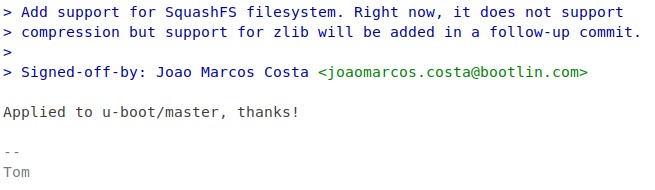
\includegraphics[scale=0.4]{figuras/tom.jpeg}
\caption{Mensagem de aceite de Tom Rini, administrador principal do U-Boot}
\end{figure}
\item Balanço final: 27 arquivos novos e/ou modificados e aproximadamente 3000 linhas de código
\end{itemize}
\end{frame}
